PWM (Pulse Width Modulation) é uma modulação baseada na conversão linear de um valor em escala de tensão para outro em escala de \emph{Duty Cicle} aplicado a uma onda quadrada de amplitude qualquer. Este tipo de modulação é essencial em controladores de circuitos de potência, já que através desta modulação é possível controlar um dispositivo de chaveamento como um Mosfet,  de modo que a tensão média sobre uma dada carga esteja diretamente relacionada com \emph{Duty Cicle} do chaveamento.  

\section{Modos de Funcionamento}

Para criar uma modulação PWM é necessário criar uma onda portadora cuja a amplitude do sinal varie no tempo permitindo compara a sua amplitude com o do sinal modulante. O sinal modulante nada mais é do que o sinal ao qual se deseja converter em escala de \emph{Duty Cicle}. Normalmente a onda portadora utilizada neste tipo de modulação é a onda triangular ou a onda dente de serra.  

\begin{figure}[H]
	\centering
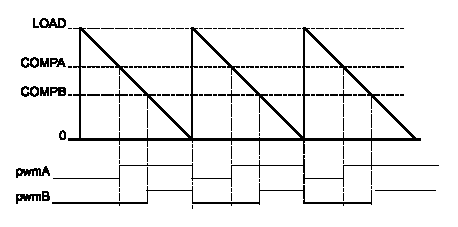
\includegraphics[width=0.8\textwidth] {figuras/Down.eps}
	\caption{PWM modo Down \cite{DATASHEET_TIVA}}
	\label{fig:Down}
\end{figure}

\begin{figure}[H]
	\centering
	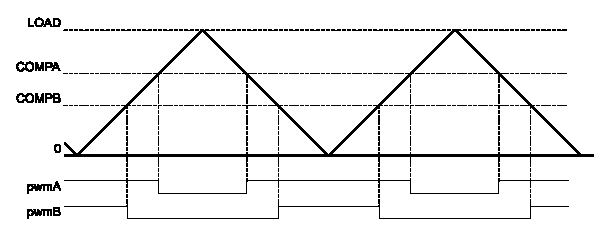
\includegraphics[width=0.8\textwidth] {figuras/UpDown.eps}
	\caption{PWM modo Down \cite{DATASHEET_TIVA}}
	\label{fig:UpDown}
\end{figure}

\section{PWM do TM4C1294NCPDT}

\begin{figure}[H]
	\centering
	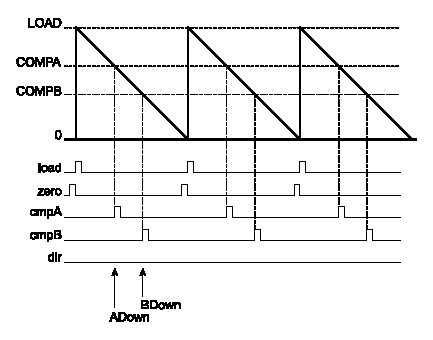
\includegraphics[width=0.8\textwidth] {figuras/PWMCountDownMode.eps}
	\caption{PWM modo Down \cite{DATASHEET_TIVA}}
	\label{fig:PWMCountDownMode}
\end{figure}

\begin{figure}[H]
	\centering
	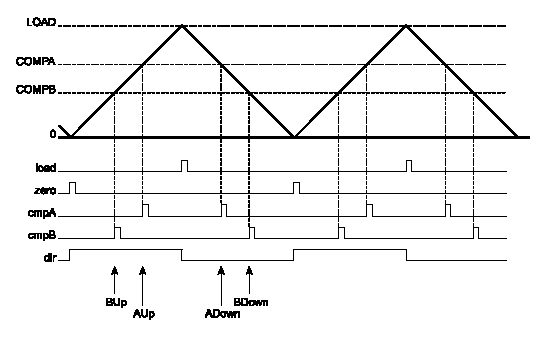
\includegraphics[width=0.8\textwidth] {figuras/PWMCountUpDownMode.eps}
	\caption{PWM modo Down \cite{DATASHEET_TIVA}}
	\label{fig:PWMCountUpDownMode}
\end{figure}